\documentclass[10pt,leter,openany]{article}
\usepackage[utf8]{inputenc}
\usepackage[spanish]{babel}
\usepackage{amsmath}
\usepackage{amsfonts}
\usepackage{amssymb}
\usepackage{graphicx}
\usepackage{listings}
\usepackage{color}
\usepackage[left=3cm,right=3cm,top=3cm,bottom=3cm]{geometry}
\usepackage[numbers,sort&compress]{natbib}
\usepackage{url}
\usepackage{caption}
\usepackage{siunitx}
%\usepackage{subfigure}
\usepackage{float}
\usepackage{booktabs}
\usepackage{subcaption}
\usepackage{mwe}
\usepackage{comment}

\setlength{\parindent}{0pt}
\setlength{\parskip}{4pt}

\usepackage{pdfpages}

\begin{document}
	
	\thispagestyle{empty}
\vspace{10 cm}
\begin{scshape}
\begin{center}
	{$\,$} \\[20 mm]
	{\Large{Universidad Autónoma de Nuevo León}} \\[5mm]
	{\large{Facultad de Ingeniería Mecánica y Eléctrica}} \\[5mm]
	{\large{Posgrado en Ingeniería de Sistemas}} \\[5 mm]
	{\large{Doctorado}}
	\vskip16mm
	\begin{figure}[h!]
		\centering
		\begin{subfigure}{0.3\linewidth}
			
\includegraphics[width=\linewidth]{fig/uanl}
		\end{subfigure}
		\hspace{15 mm}
		\begin{subfigure}{0.2\linewidth}
			
\includegraphics[width=\linewidth]{fig/fime}
		\end{subfigure}
	\end{figure}
	\vskip16mm
	\begin{tabular}{p{11cm}}
		\centering
		{\large Portafolio de Evidencias}
	\end{tabular}
	\vskip7mm
	{de}\\[7mm]
	{\large Oscar Alejandro Hernández López}\\[3mm]
	{1985273}\\[7 mm]
	{para el curso de Modelos Probabilistas Aplicados,}\\[3mm]
	{con la profesora Dra. Elisa Schaeffer.}\\[3mm]
	Semestre Agosto 2020 - Enero 2021. \\ [5 mm]
	\url{https://github.com/oscaralejandro1907/probability-in-R}
	\vfill
\end{center}
\end{scshape}
	
\section*{Homework Assignment 1 Corrections}
	In this homework corrections in punctuantions of equations were made, added after the feedback. 
	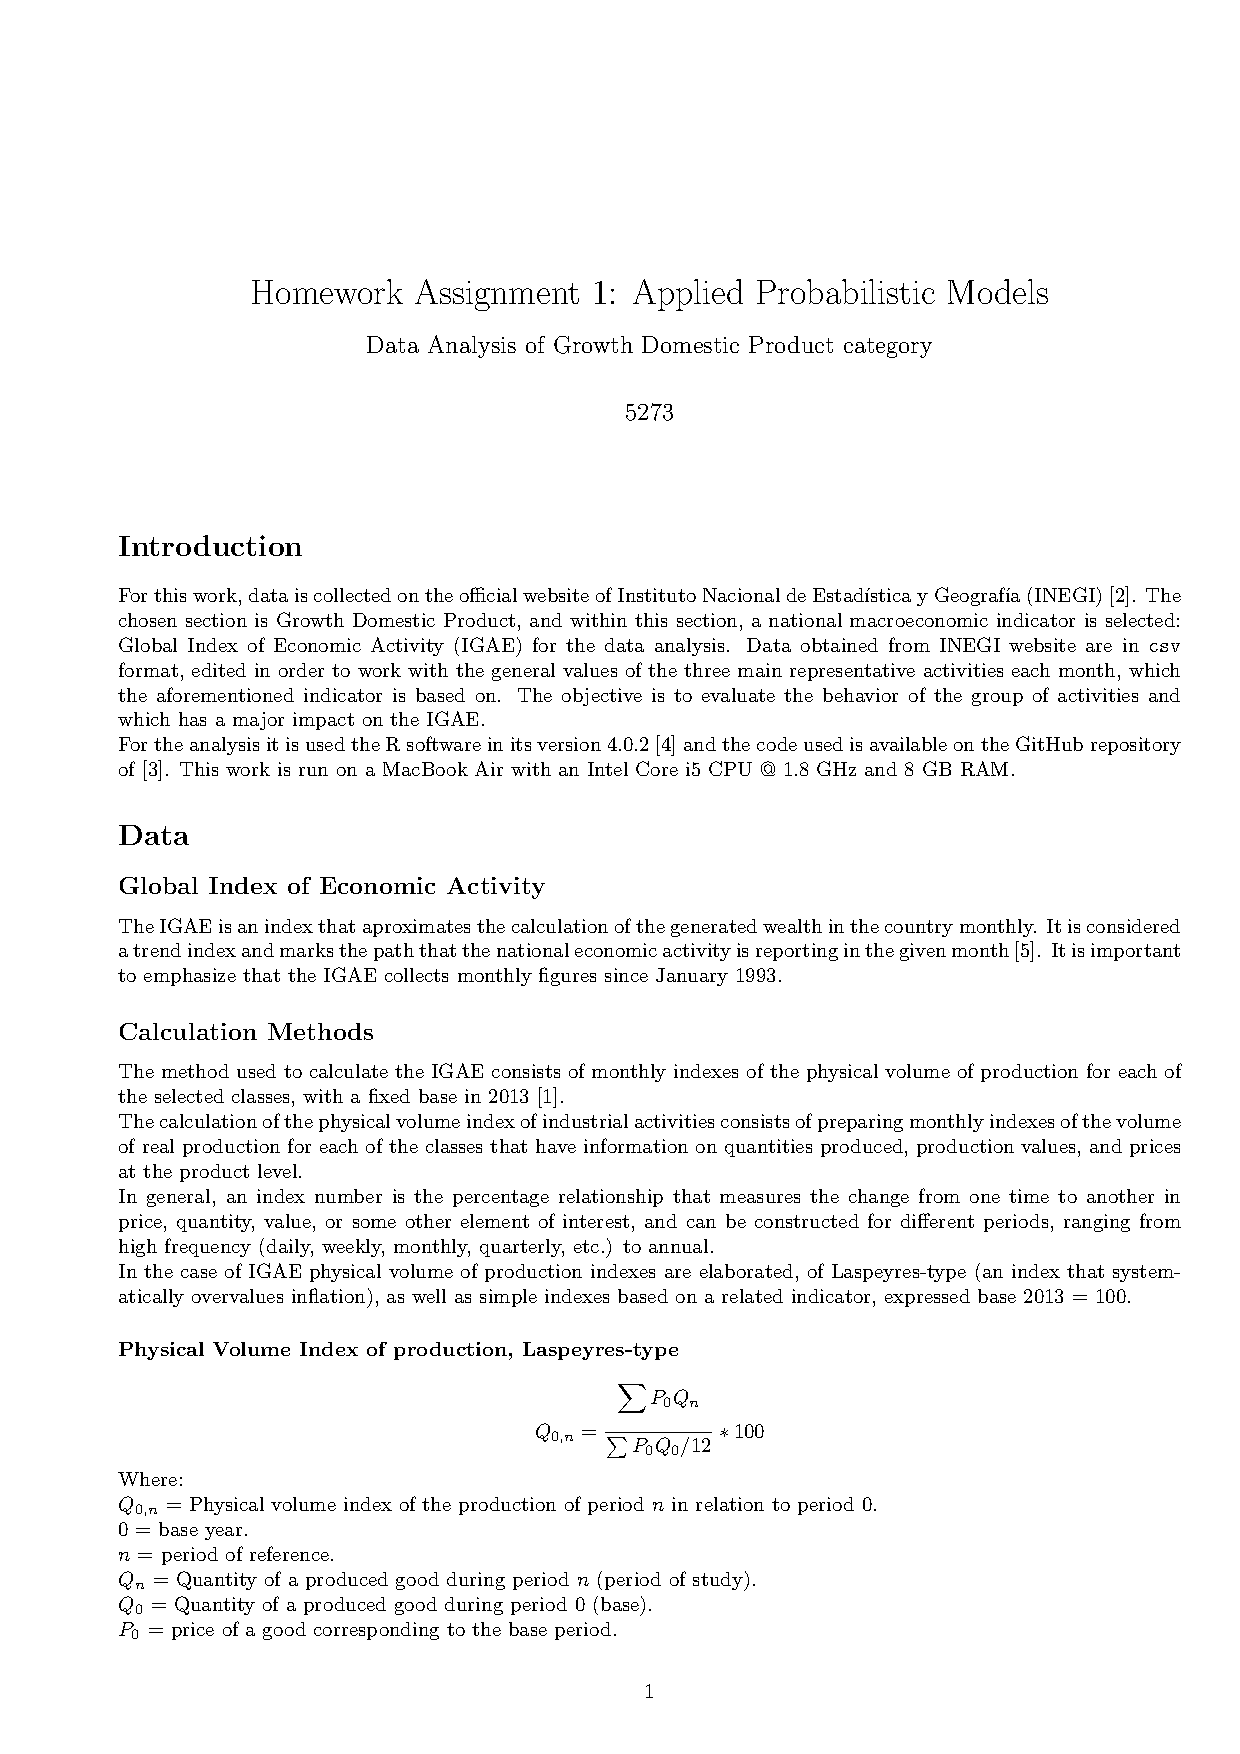
\includepdf[pages=-]{/Users/oscarhernandezlopez/Documents/GitHub/probability-in-R/assignment01/tarea1.pdf}
	
	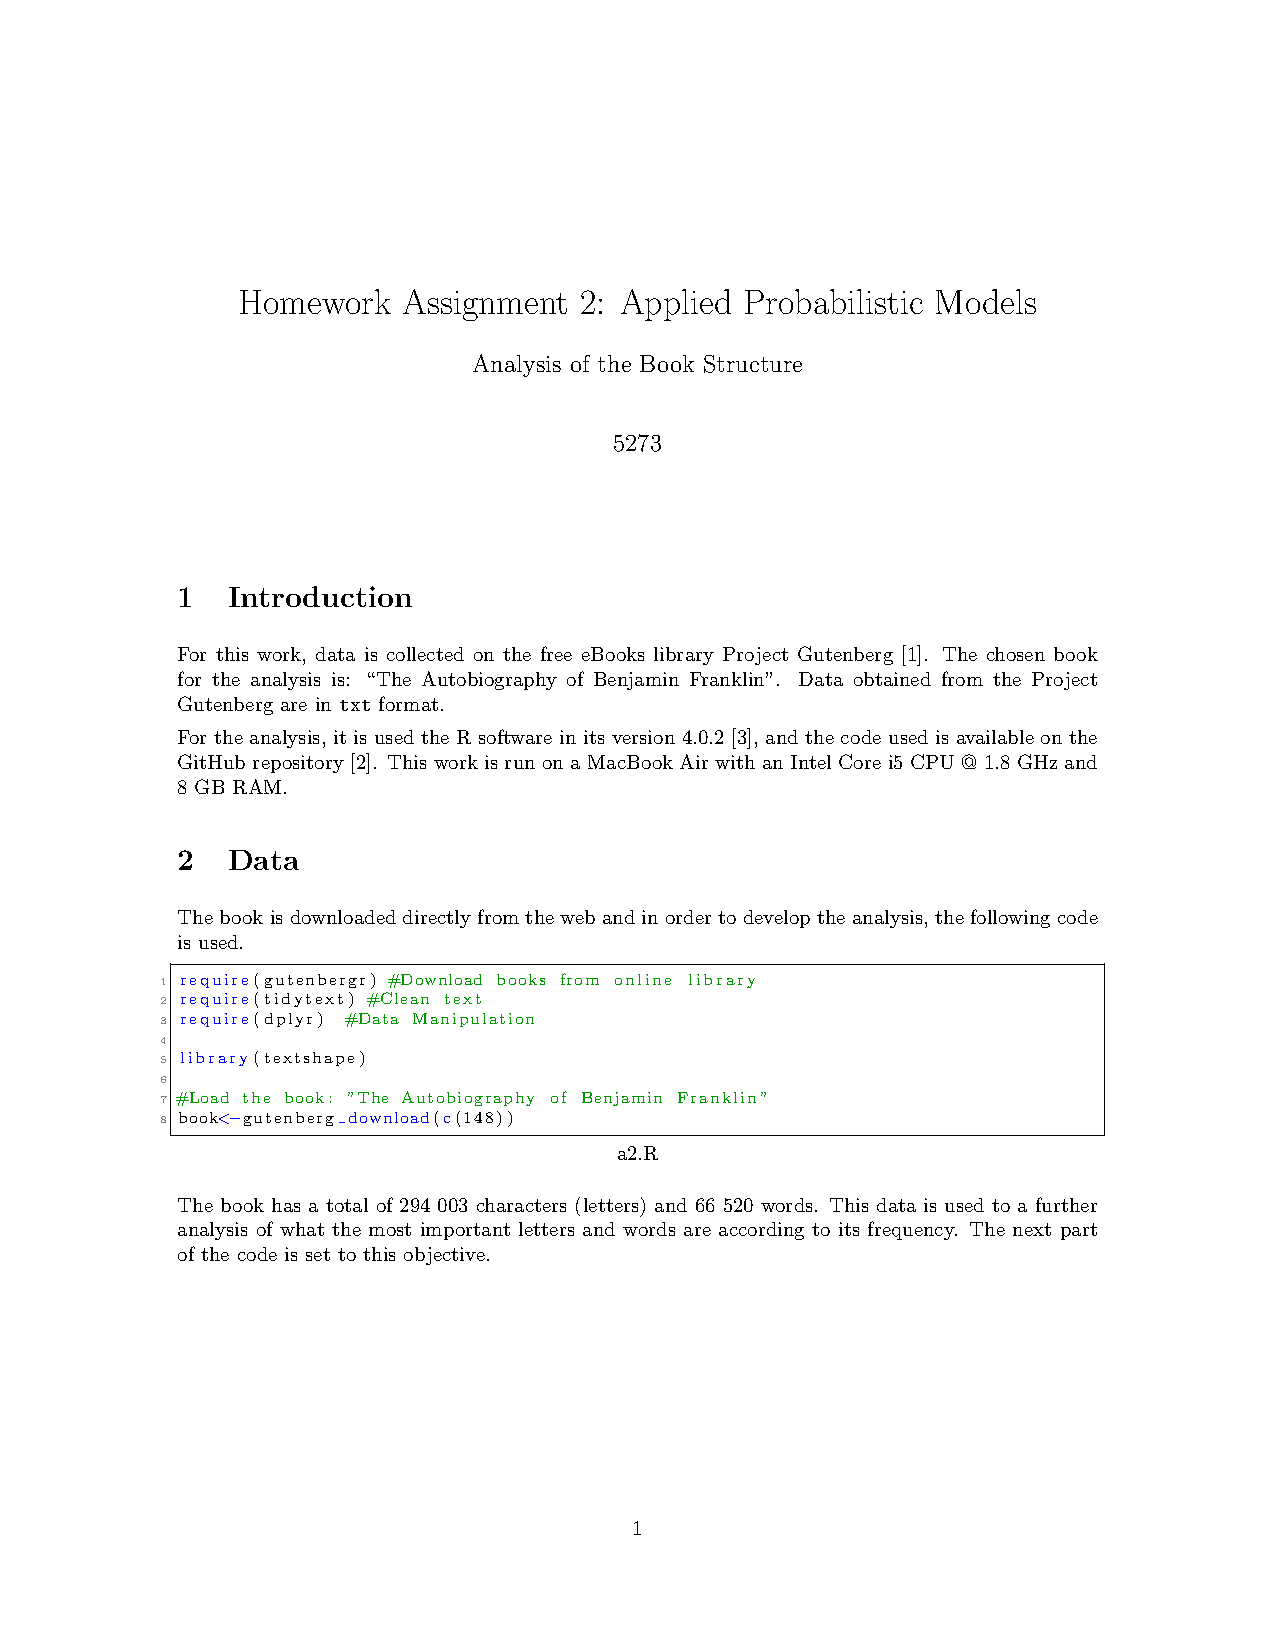
\includepdf[pages=-]{/Users/oscarhernandezlopez/Documents/GitHub/probability-in-R/assignment02/assignment2.pdf}
	
	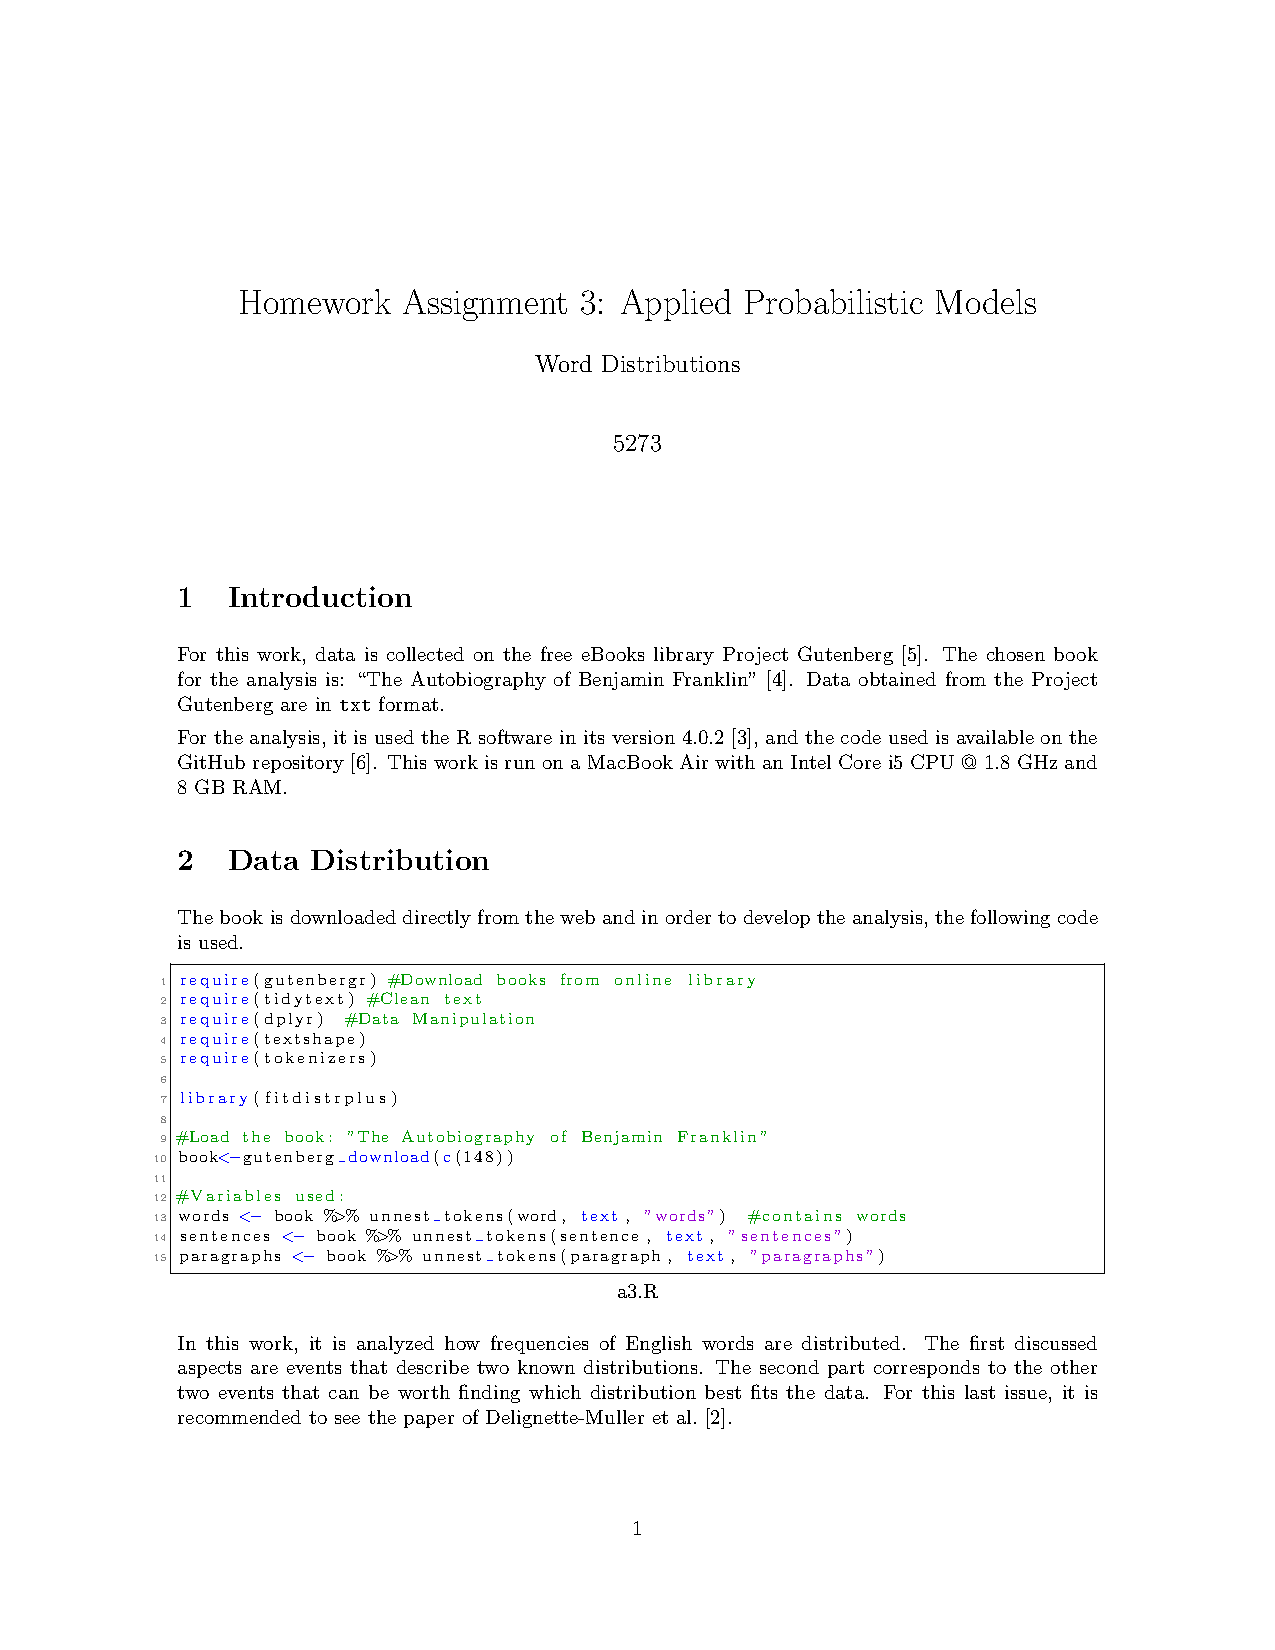
\includepdf[pages=-]{/Users/oscarhernandezlopez/Documents/GitHub/probability-in-R/assignment03/assignment3.pdf}
	
	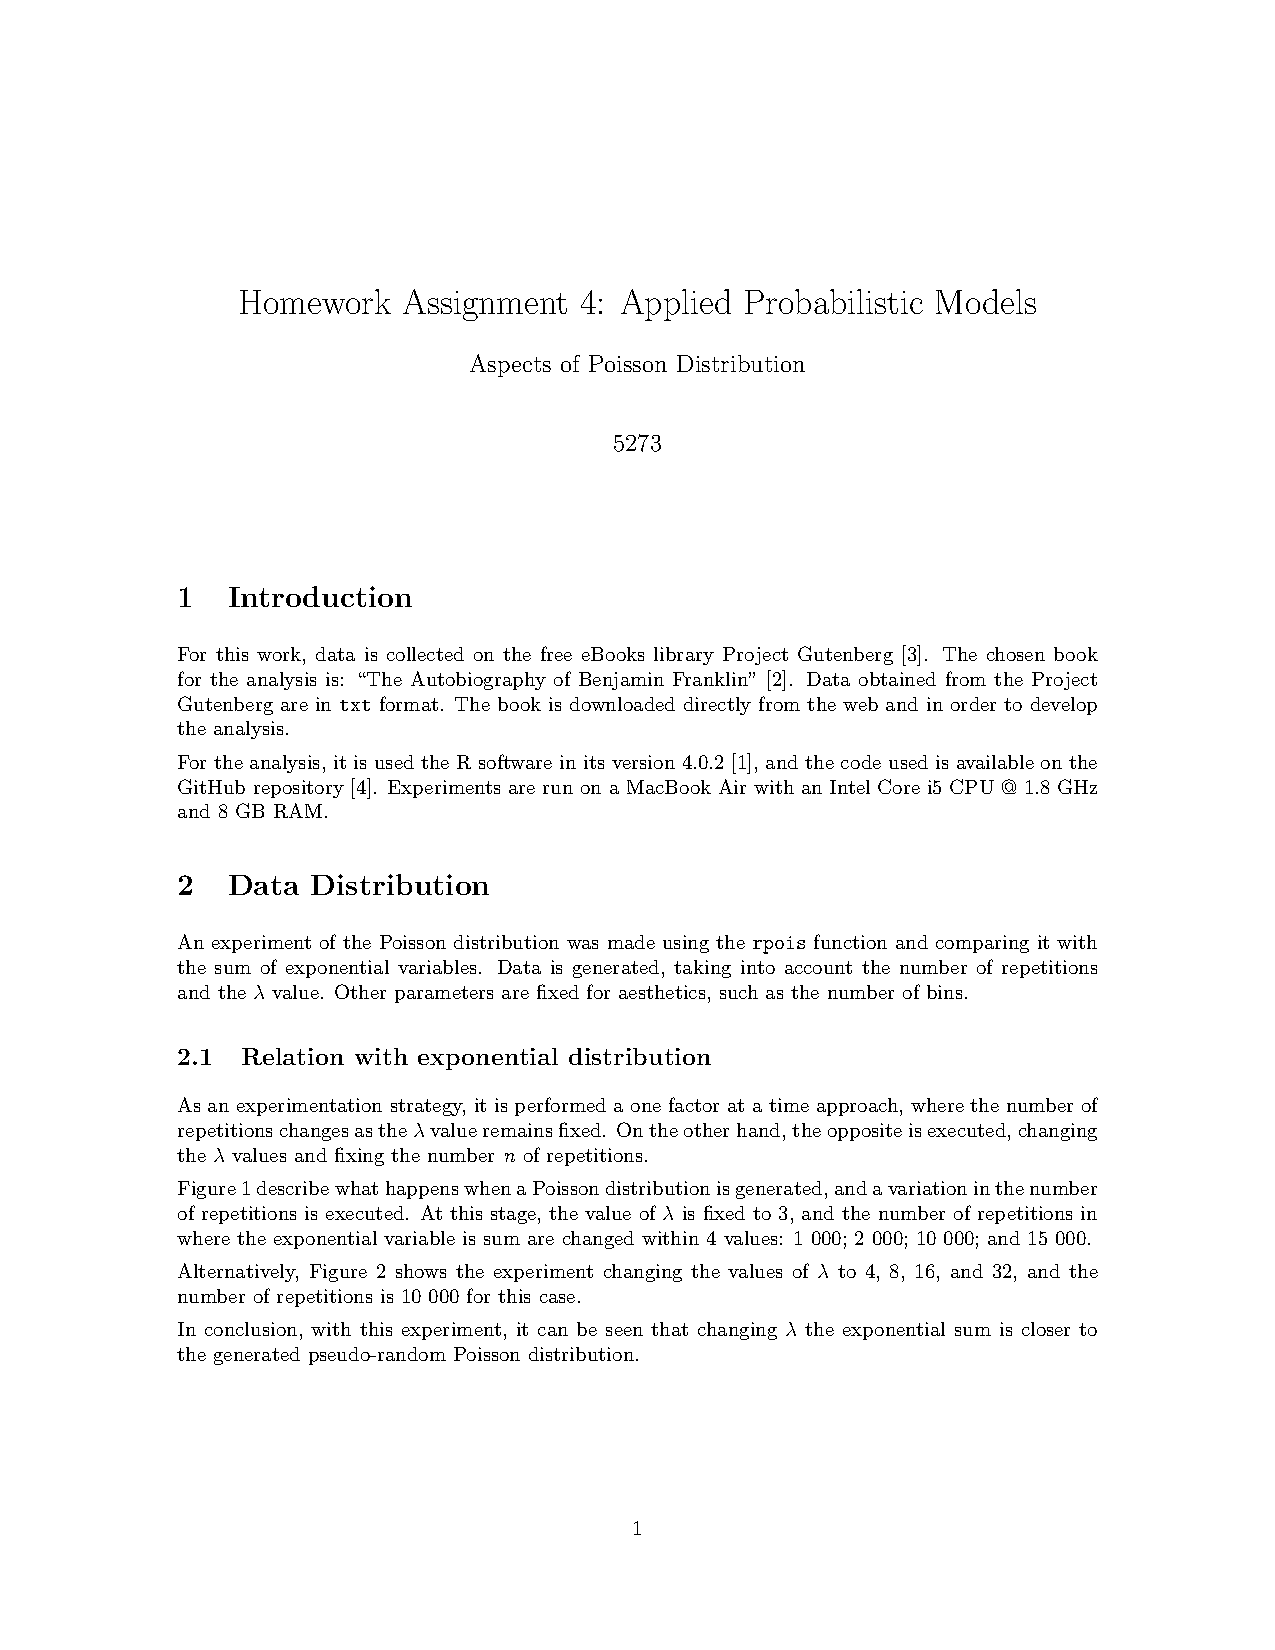
\includepdf[pages=-]{/Users/oscarhernandezlopez/Documents/GitHub/probability-in-R/assignment04/assignment4.pdf}
	
\section*{Homework Assignment 5 Corrections}
	In this homework, data corresponding to smaller $p$-values were rewritten to avoid confusions when interpreting the scientific notation.
	
	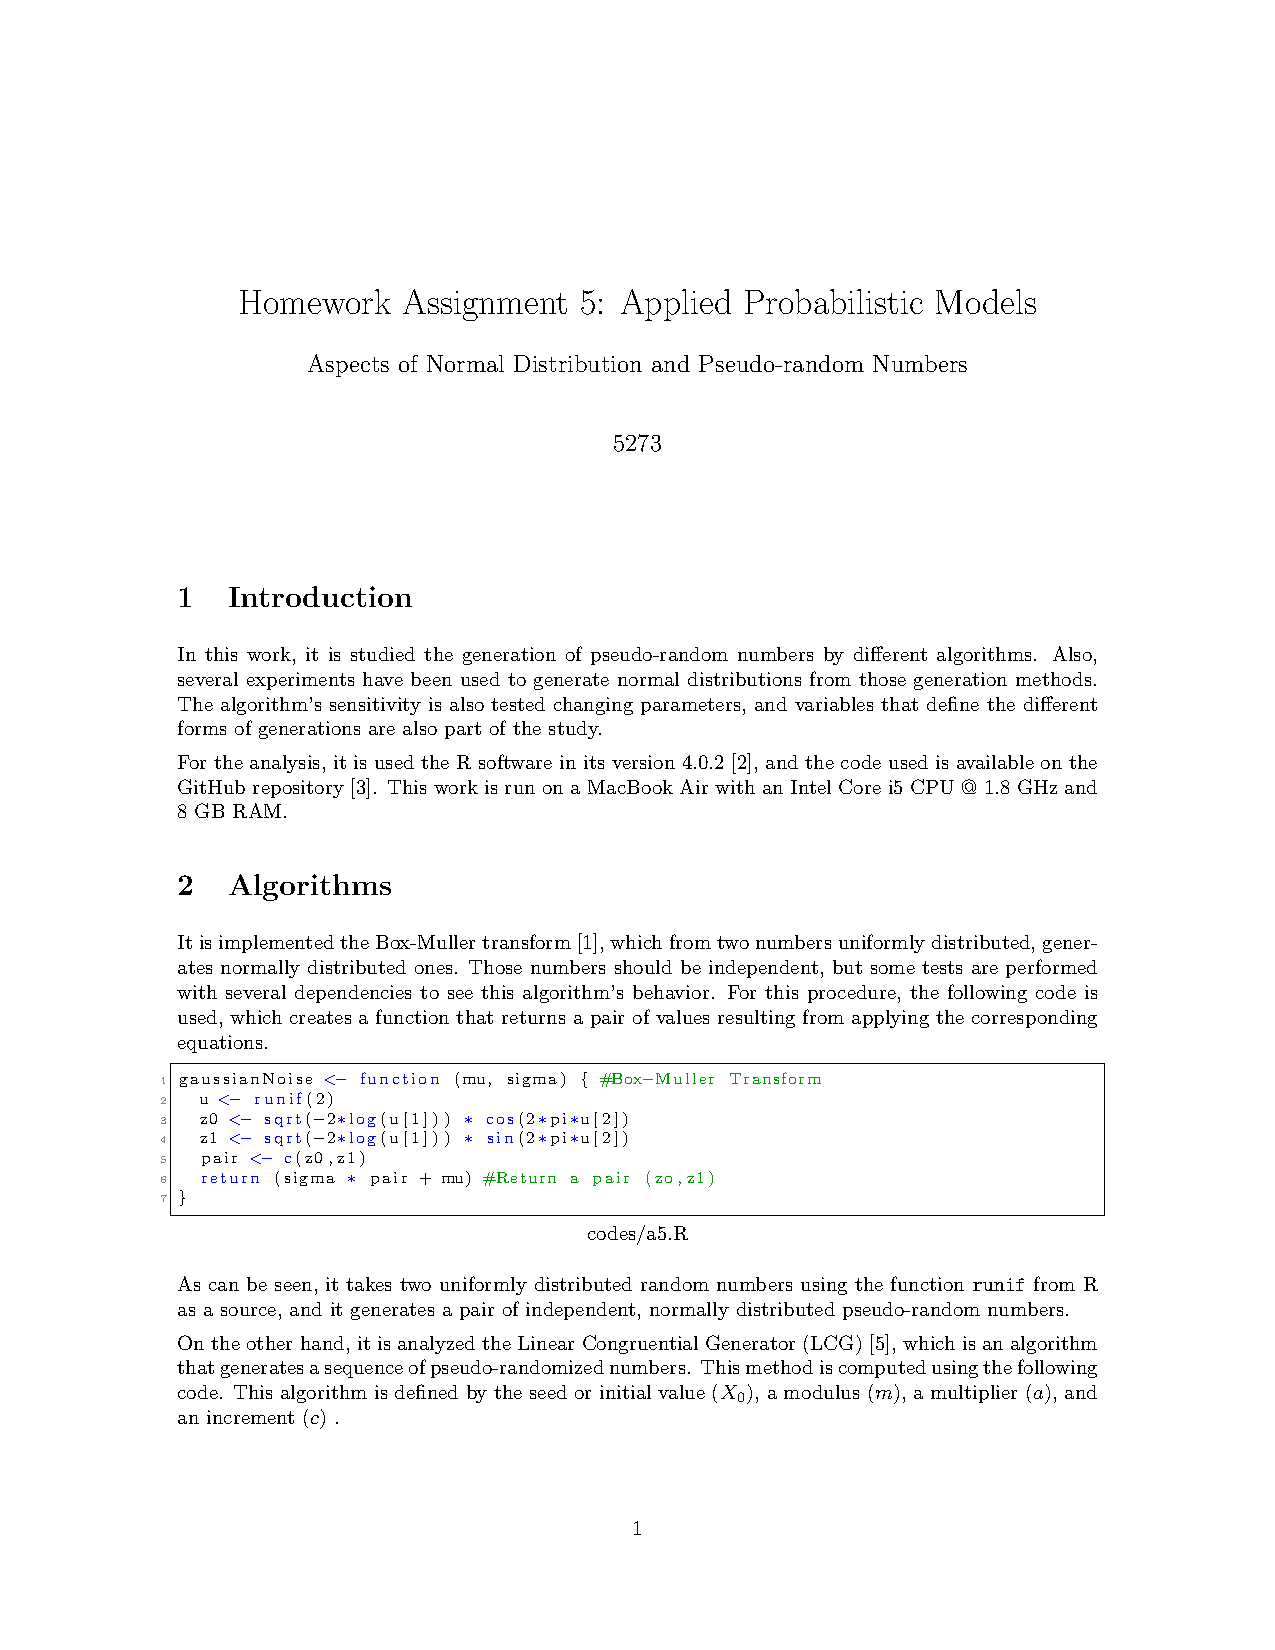
\includepdf[pages=-]{/Users/oscarhernandezlopez/Documents/GitHub/probability-in-R/assignment05/assignment5.pdf}
	
	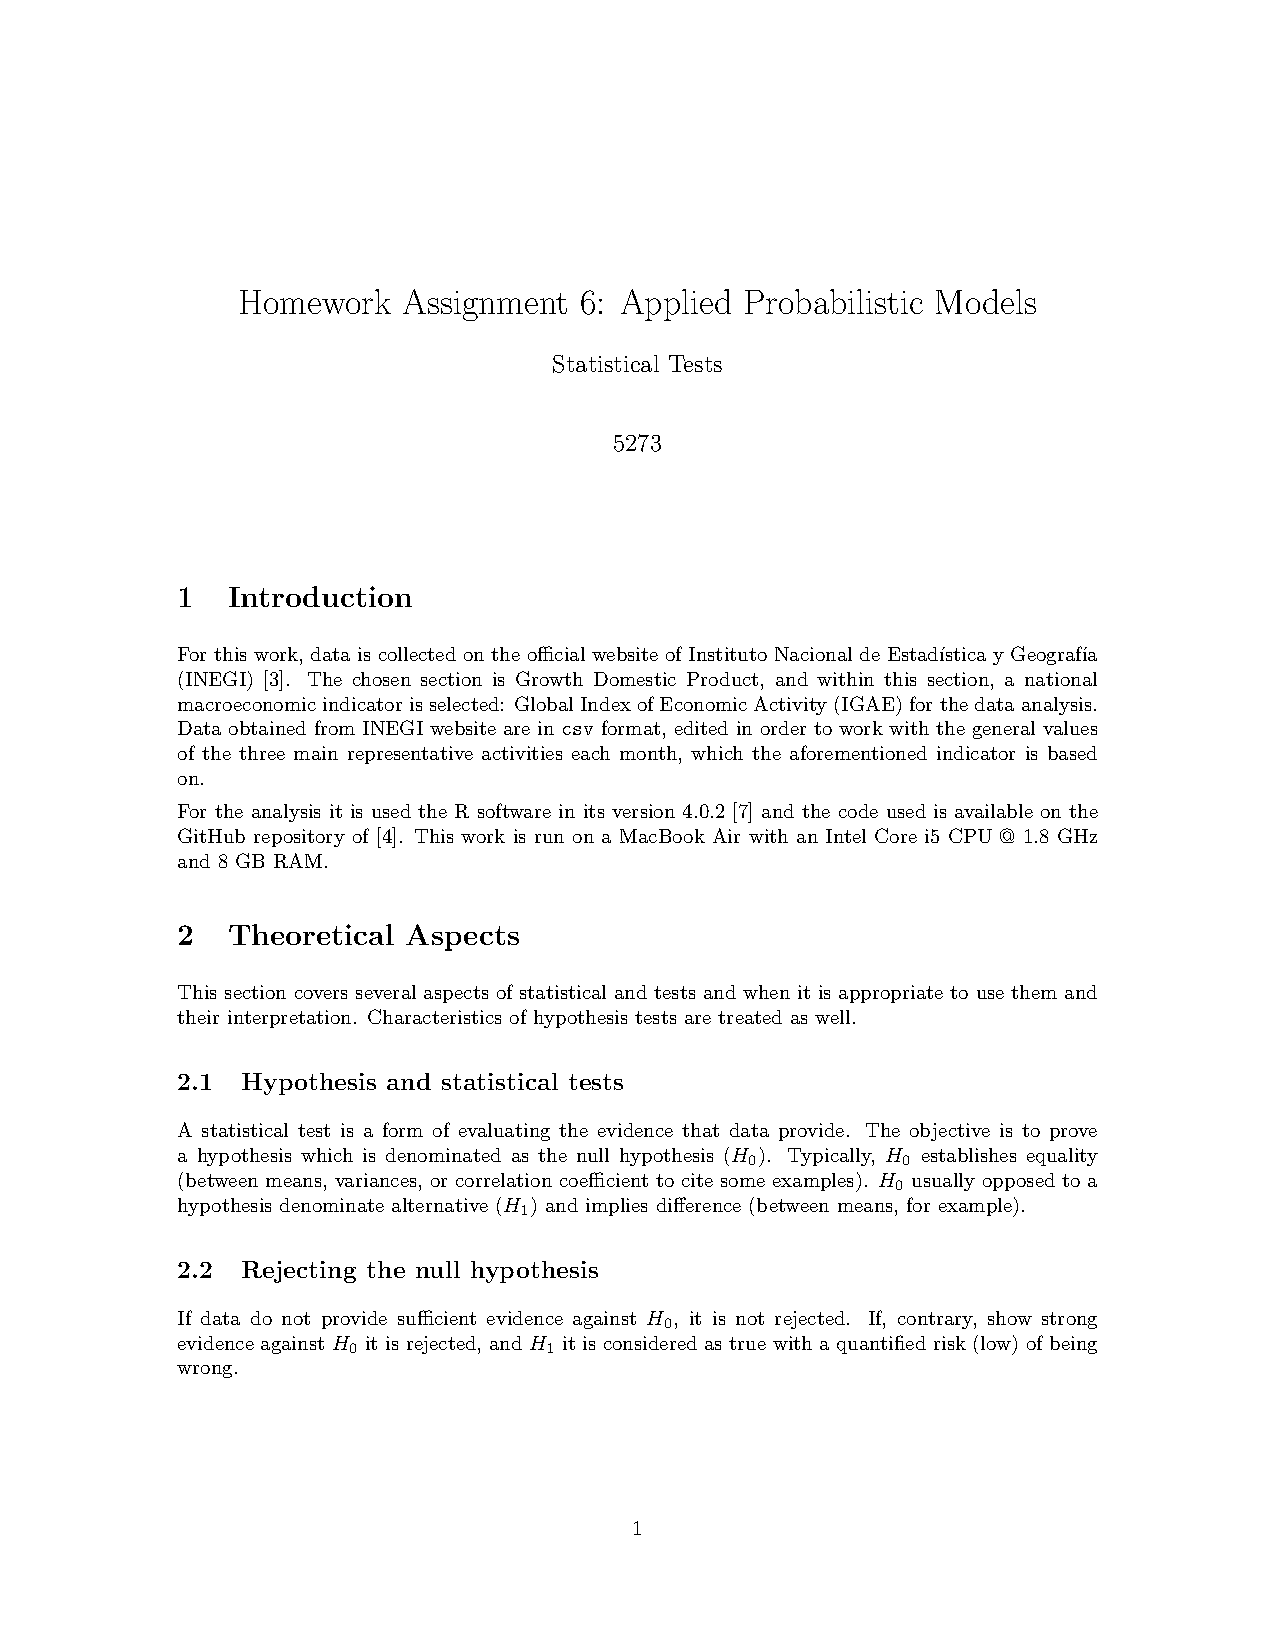
\includepdf[pages=-]{/Users/oscarhernandezlopez/Documents/GitHub/probability-in-R/assignment06/tarea6.pdf}

\section*{Homework Assignment 7 Corrections}
	In this homework, grammatical mistakes were corrected as well as some typos.
	
	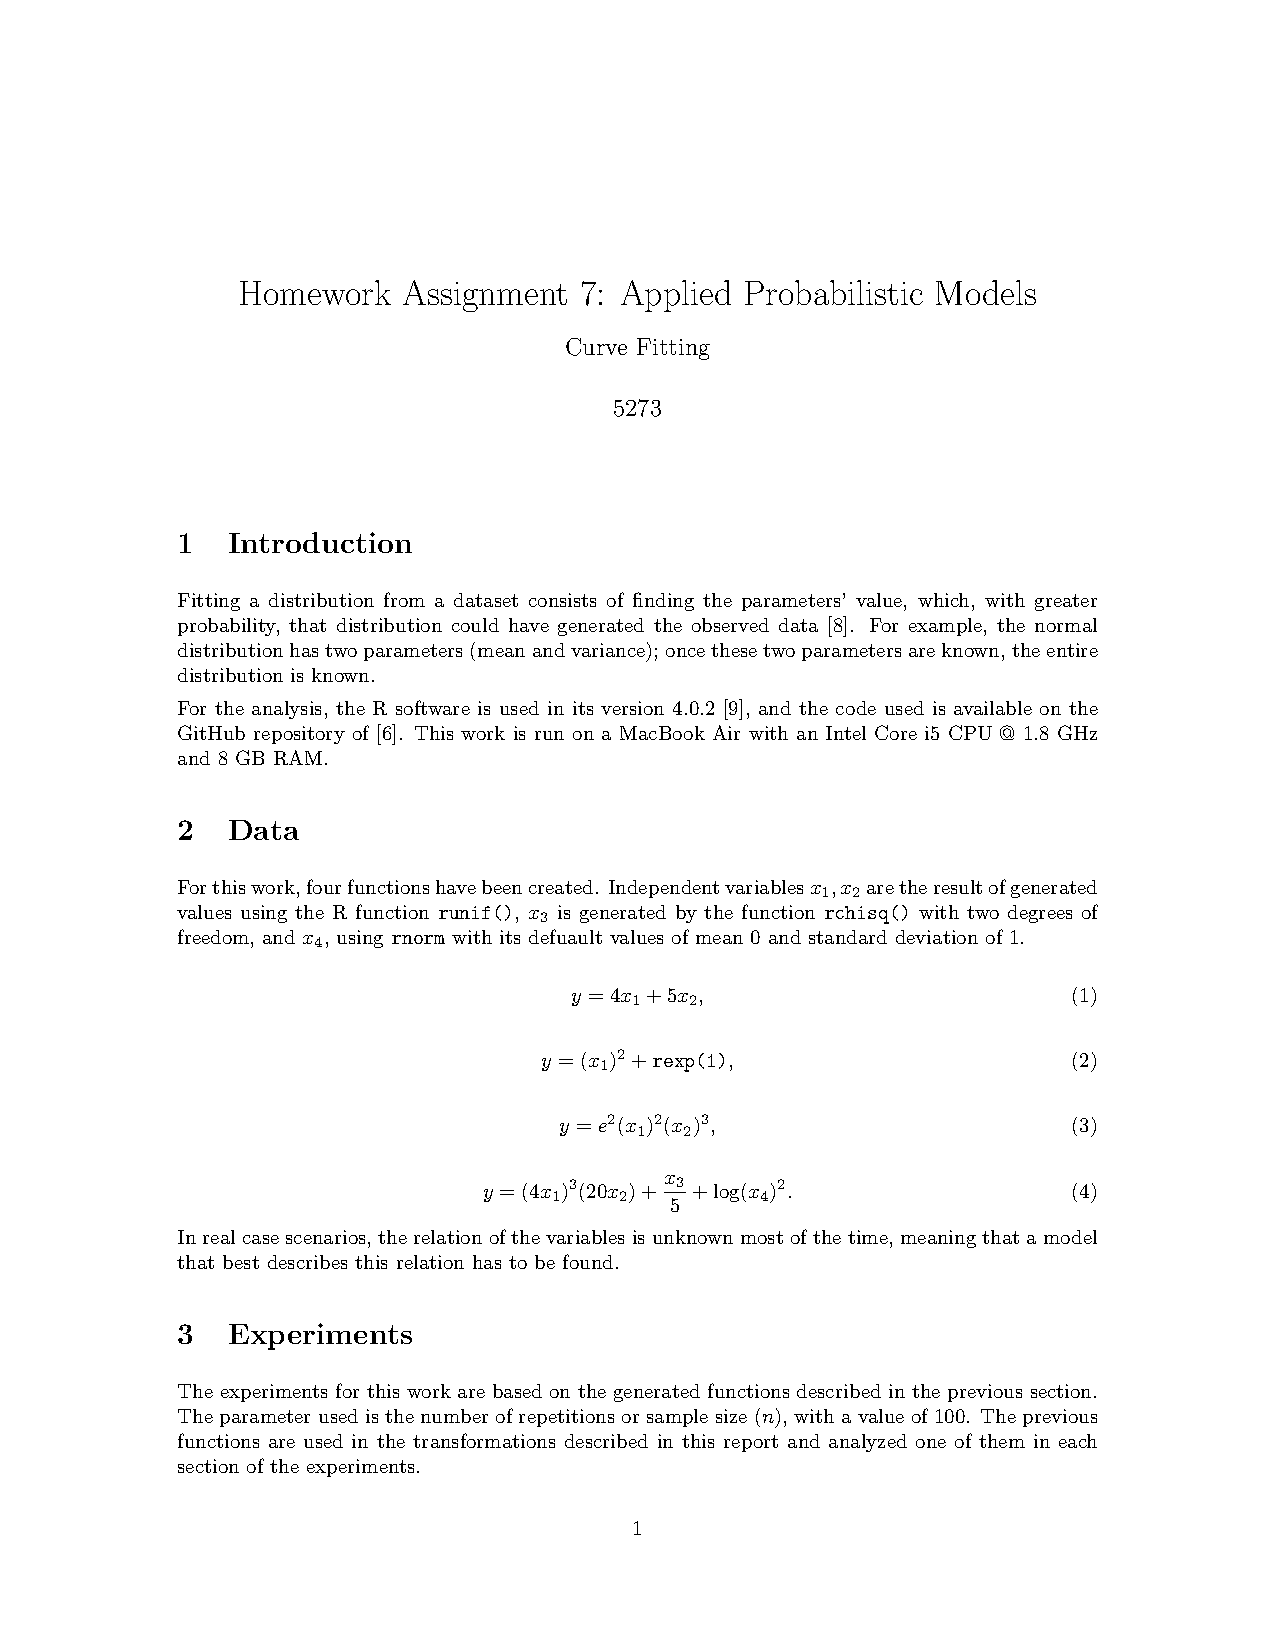
\includepdf[pages=-]{/Users/oscarhernandezlopez/Documents/GitHub/probability-in-R/assignment07/assignment7.pdf}
	
	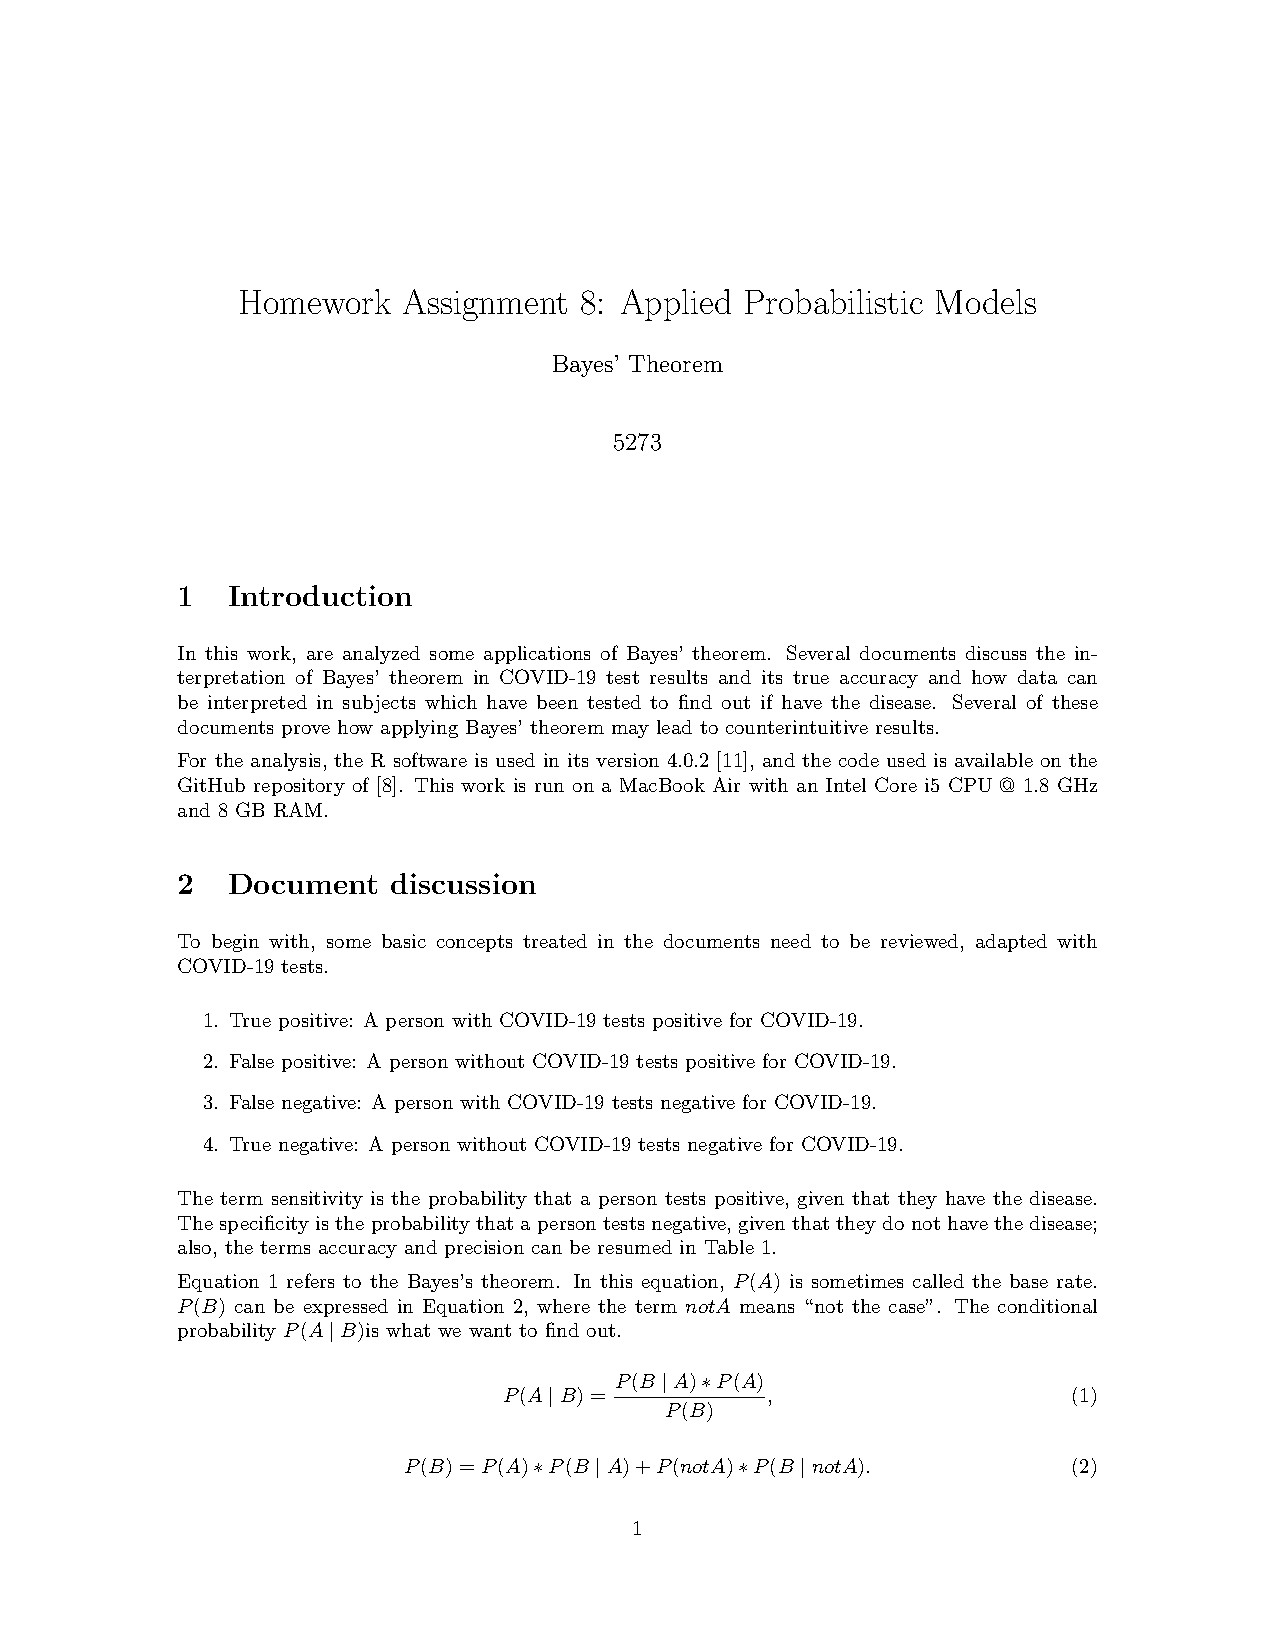
\includepdf[pages=-]{/Users/oscarhernandezlopez/Documents/GitHub/probability-in-R/assignment08/assignment8.pdf}
	
		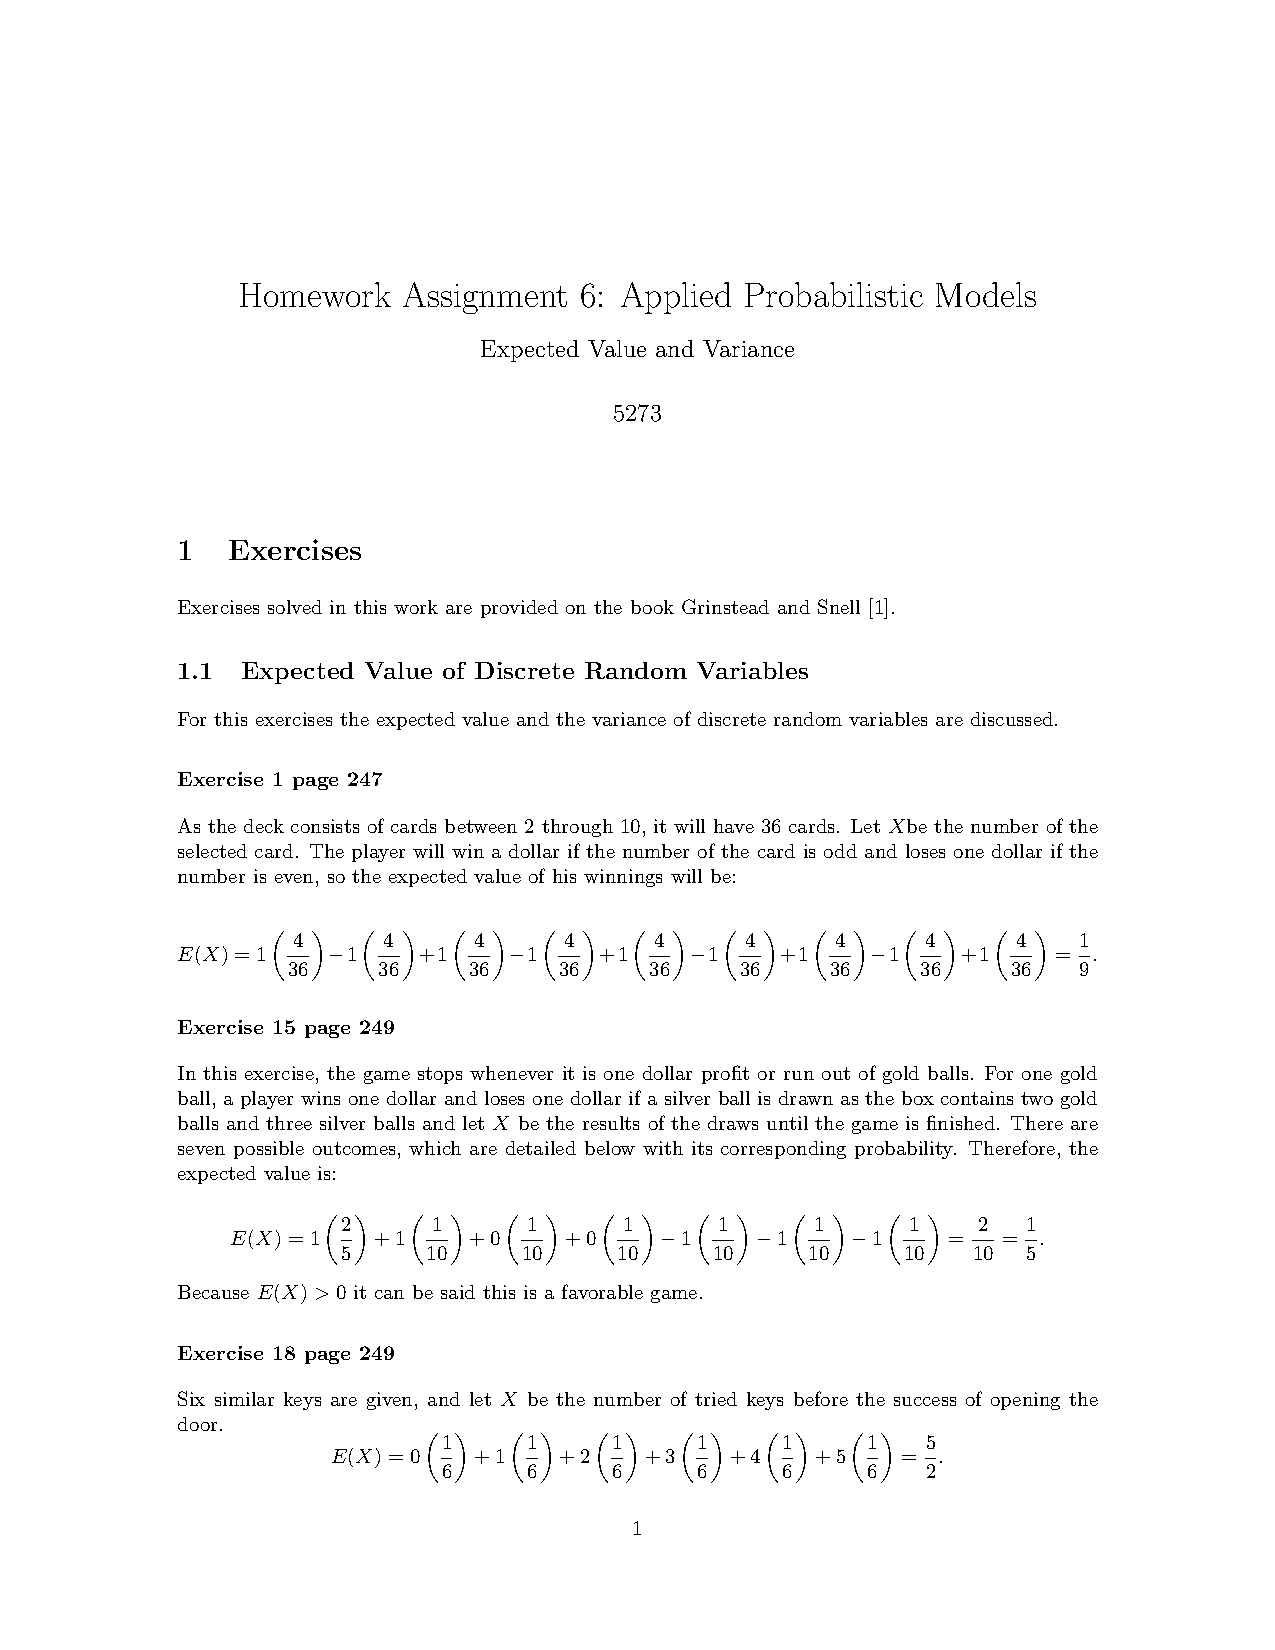
\includepdf[pages=-]{/Users/oscarhernandezlopez/Documents/GitHub/probability-in-R/assignment09/tarea9.pdf}
		
\section*{Homework Assignment 10 Corrections}
	In this homework, Exercise 18 page 249 is corrected, adjusting the number of iterations when  Monte Carlo simulation is performed, eliminating pointless iterations due to the size of the sample space. Code is modified as well.
	
	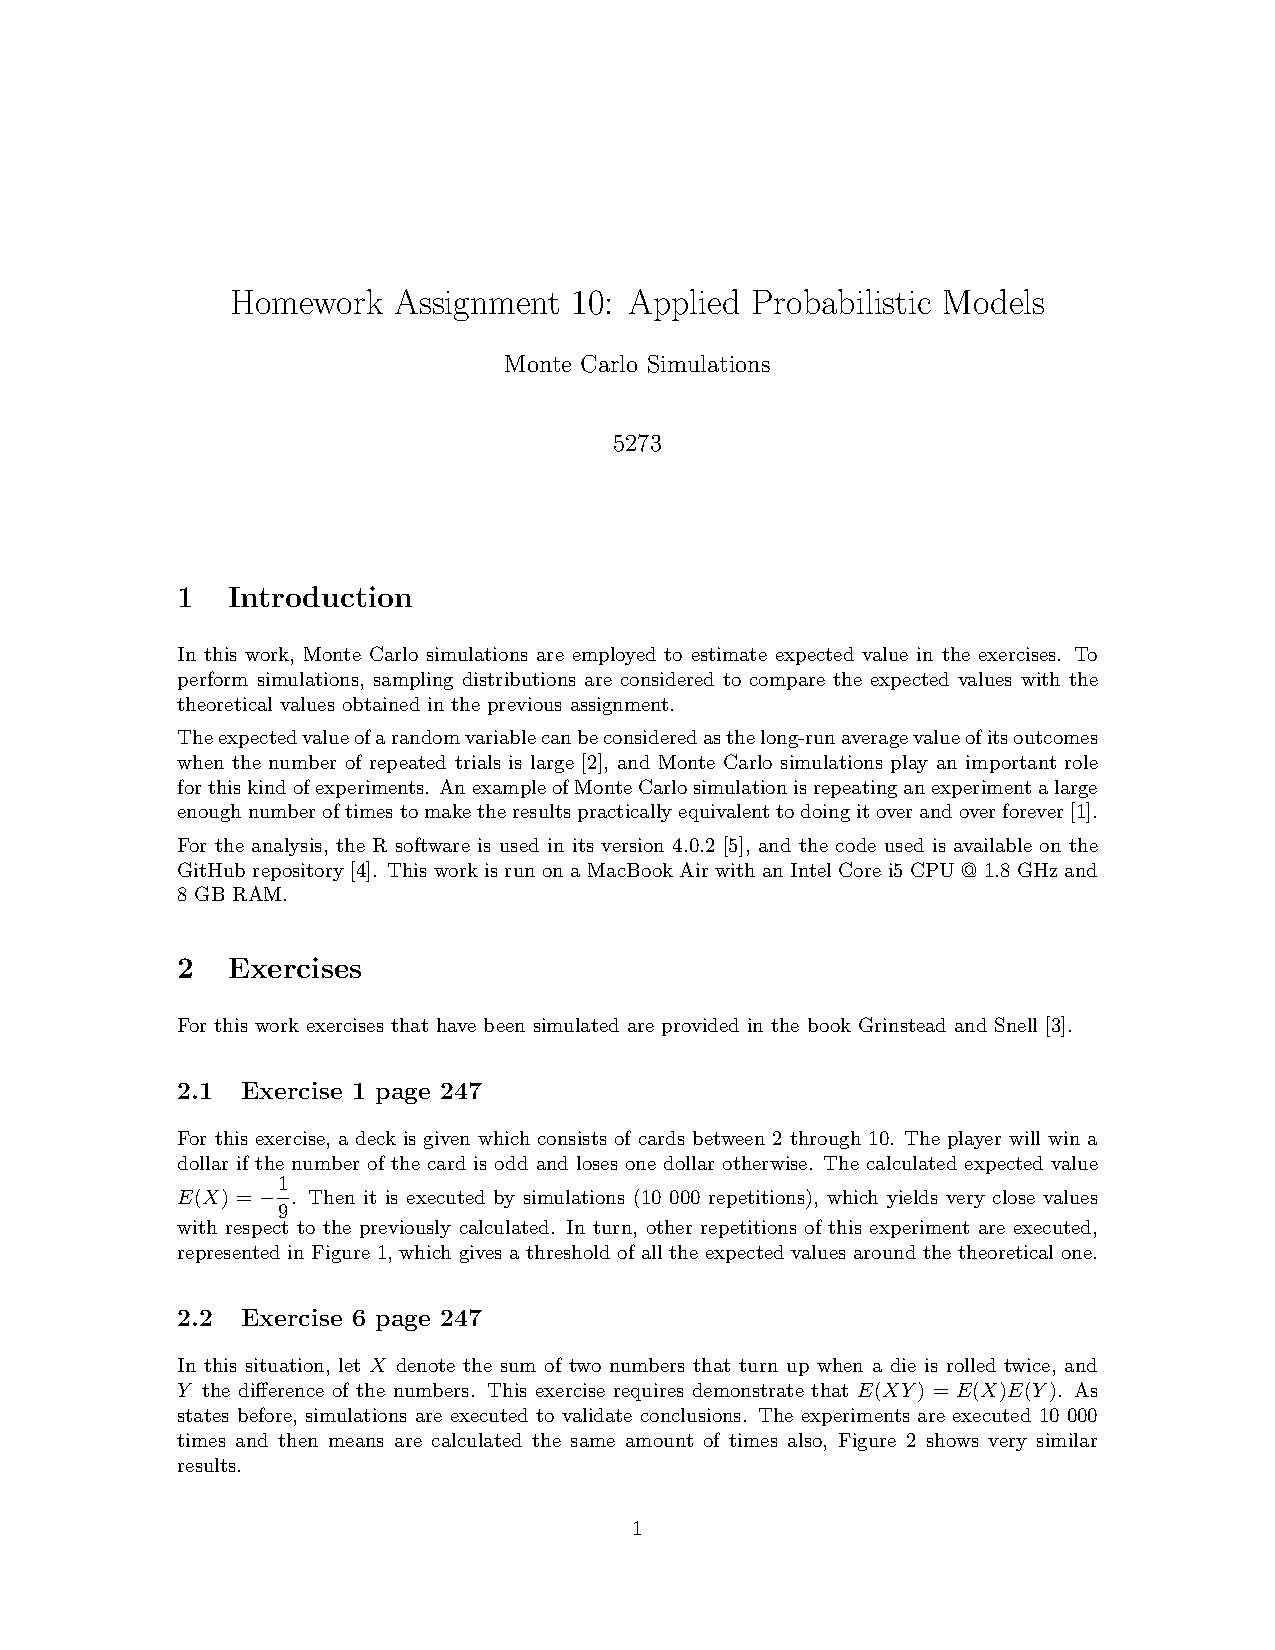
\includepdf[pages=-]{/Users/oscarhernandezlopez/Documents/GitHub/probability-in-R/assignment10/t10.pdf}
	
\section*{Homework Assignment 11 Corrections}

	In this homework, is added the demonstrations of this properties:
	\begin{itemize}
		\item $\mbox{Cov}[aX+b, cY+d] = ac\mbox{Cov}[X,Y]$,
		\item $\mbox{Var}[X+Y] = \mbox{Var}[X] + \mbox{Var}[Y] + 2\mbox{Cov}[X,Y]$.
	\end{itemize}

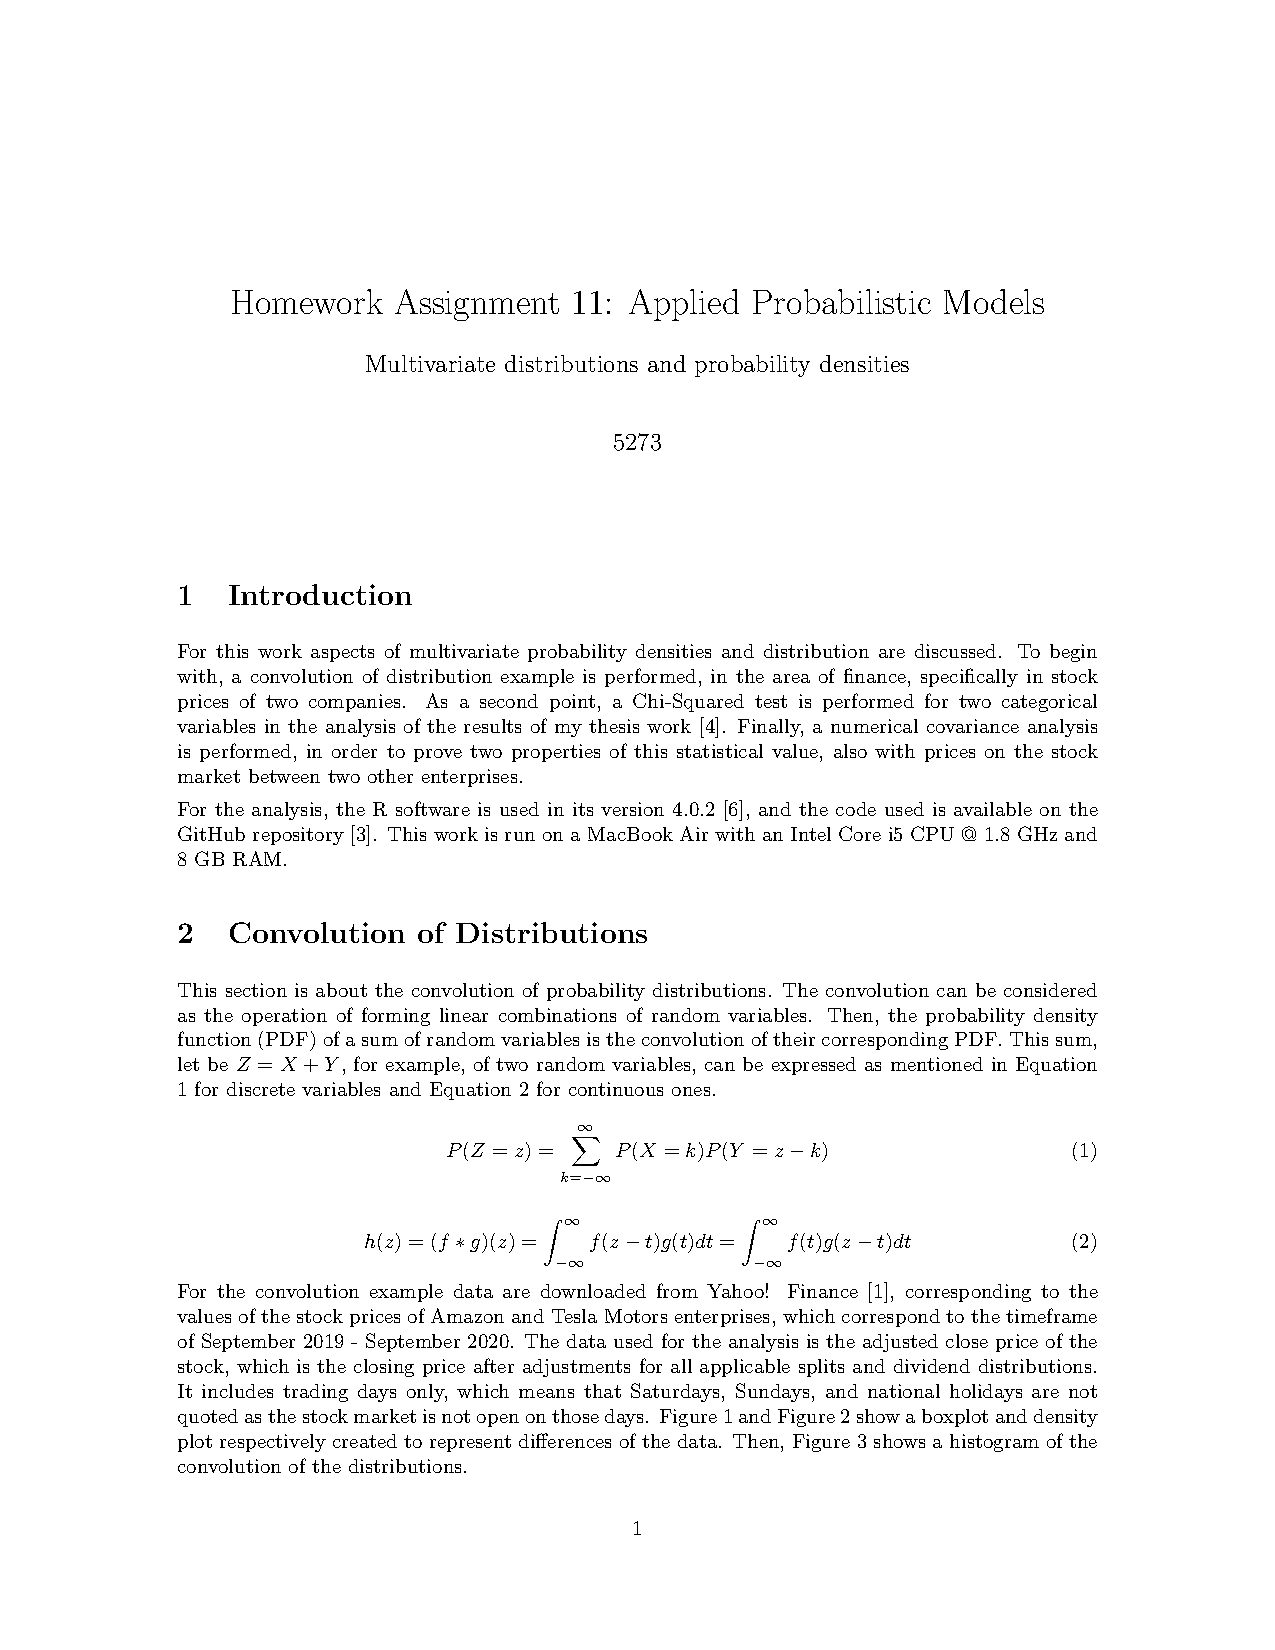
\includepdf[pages=-]{/Users/oscarhernandezlopez/Documents/GitHub/probability-in-R/assignment11/a11.pdf}

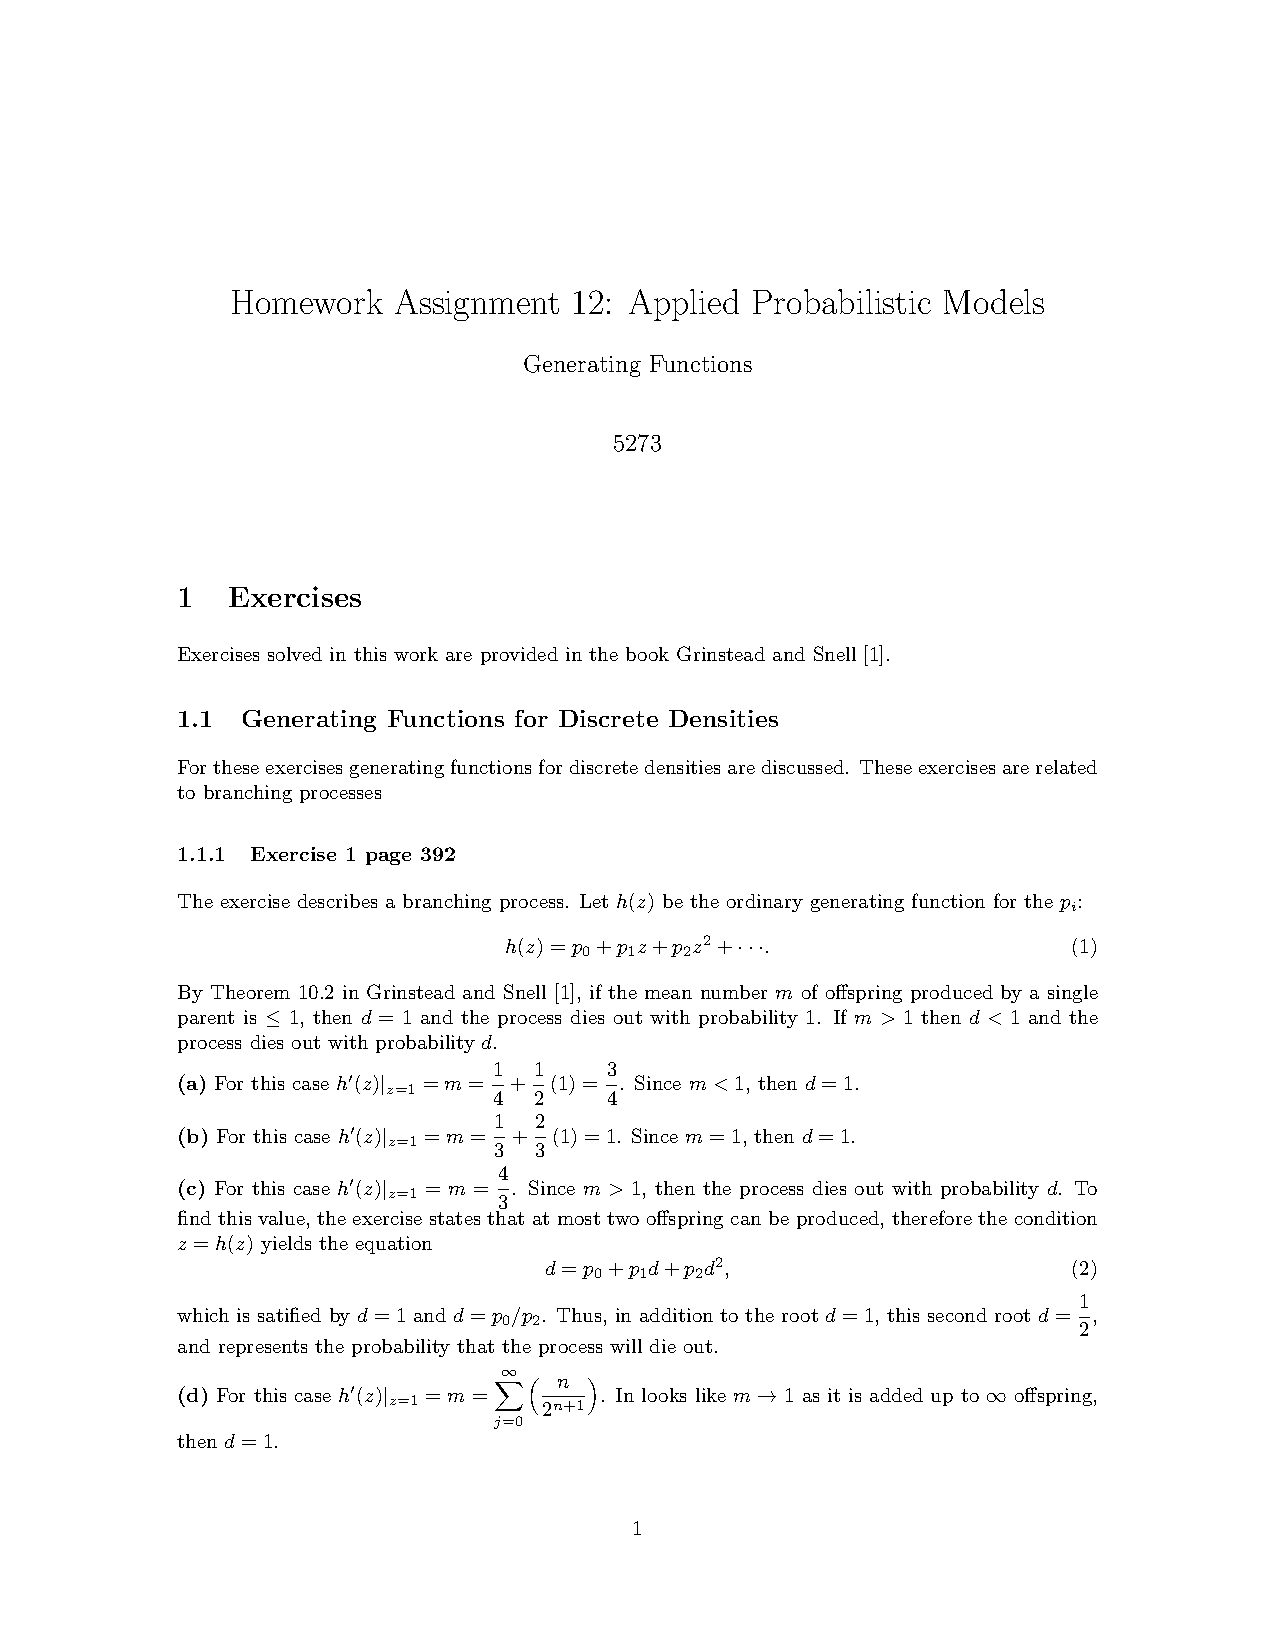
\includepdf[pages=-]{/Users/oscarhernandezlopez/Documents/GitHub/probability-in-R/assignment12/as12.pdf}

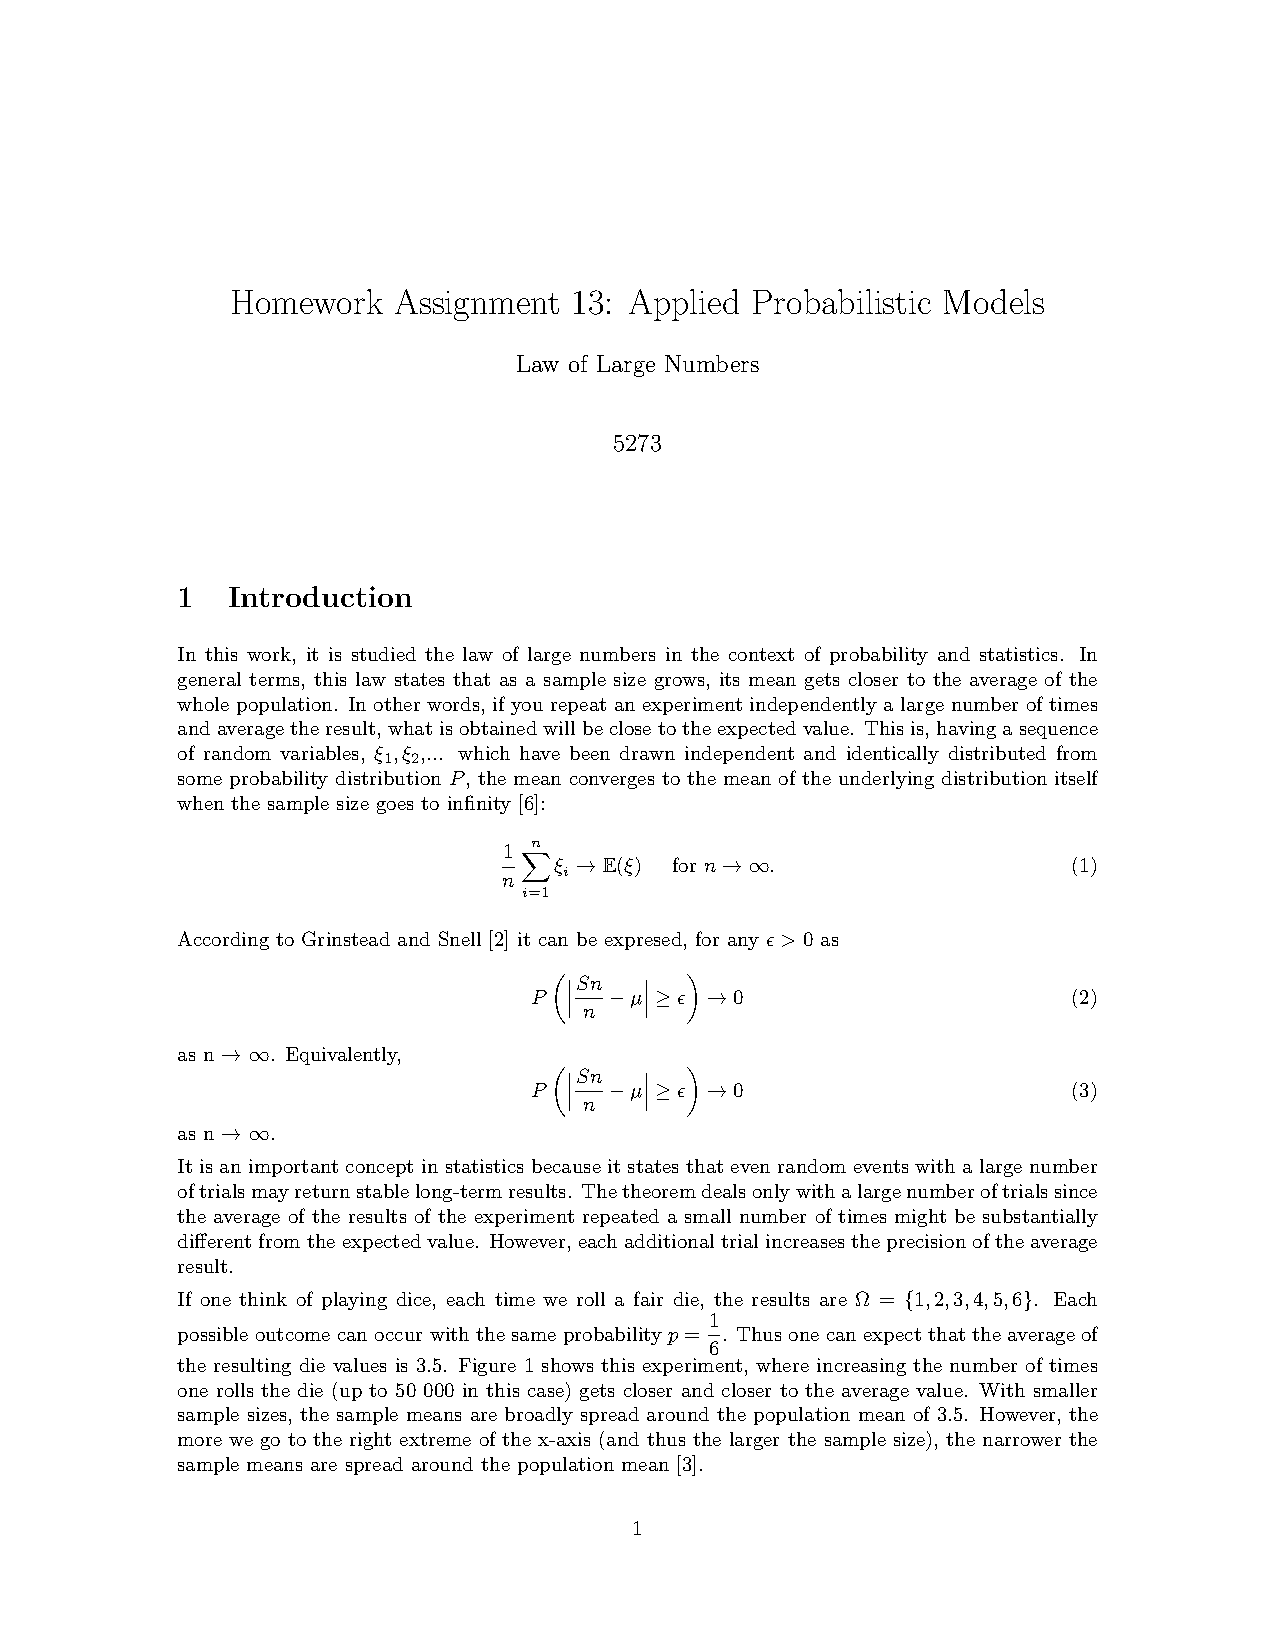
\includepdf[pages=-]{/Users/oscarhernandezlopez/Documents/GitHub/probability-in-R/assignment13/as13.pdf}

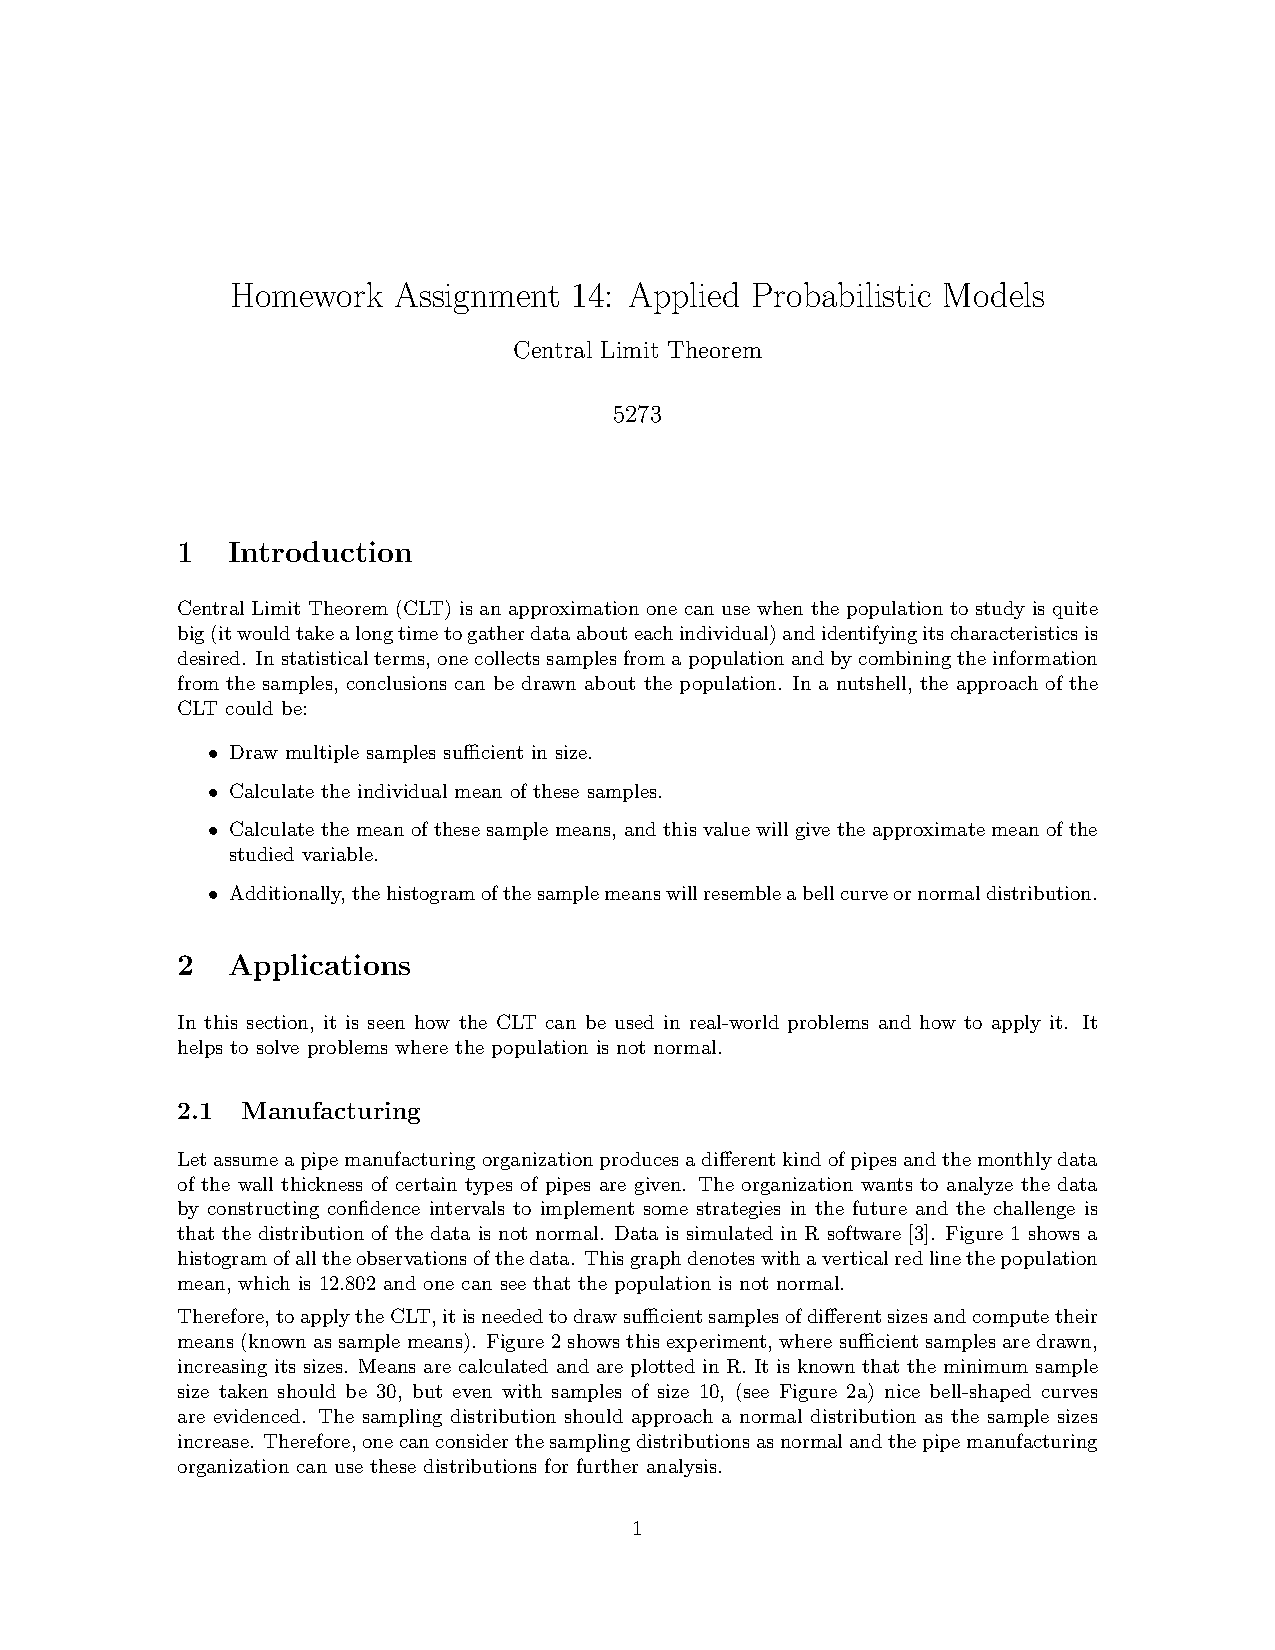
\includepdf[pages=-]{/Users/oscarhernandezlopez/Documents/GitHub/probability-in-R/assignment14/as14.pdf}

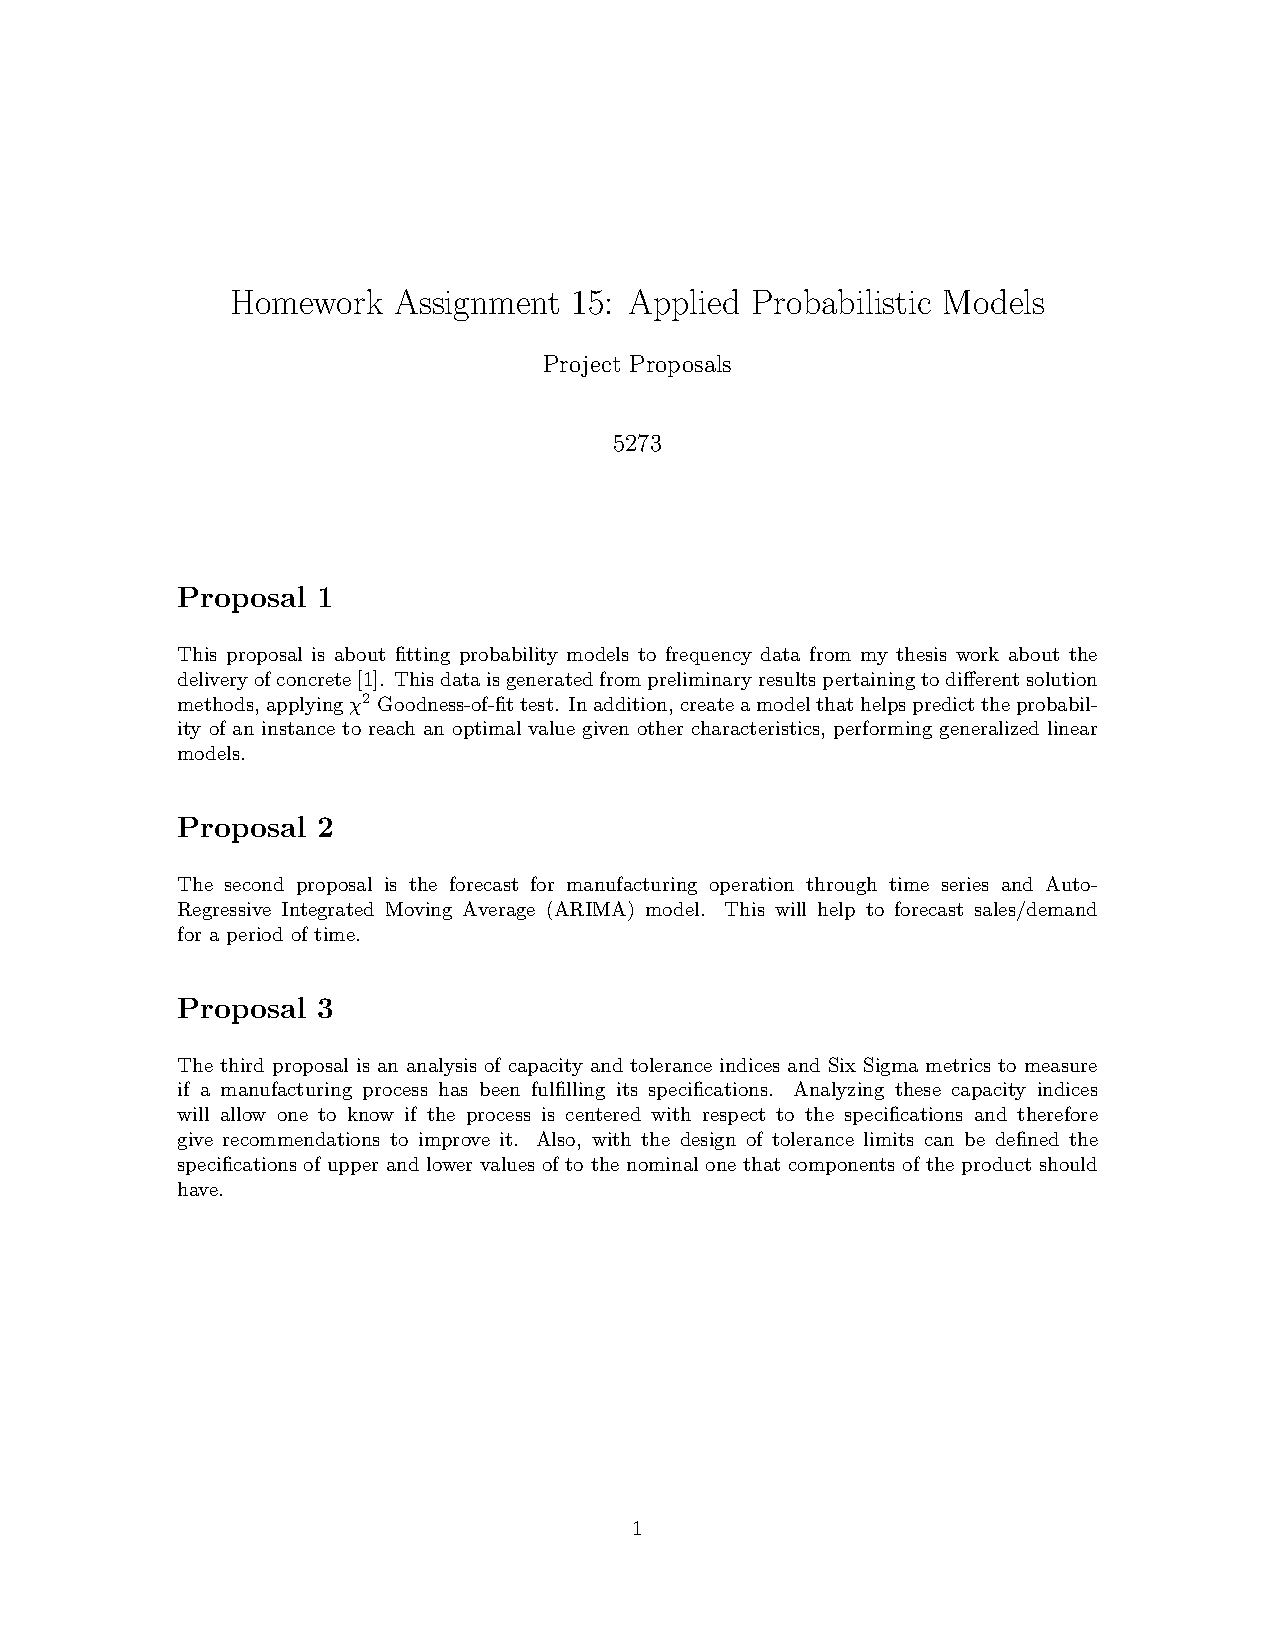
\includepdf[pages=-]{/Users/oscarhernandezlopez/Documents/GitHub/probability-in-R/assignment15/as15.pdf}

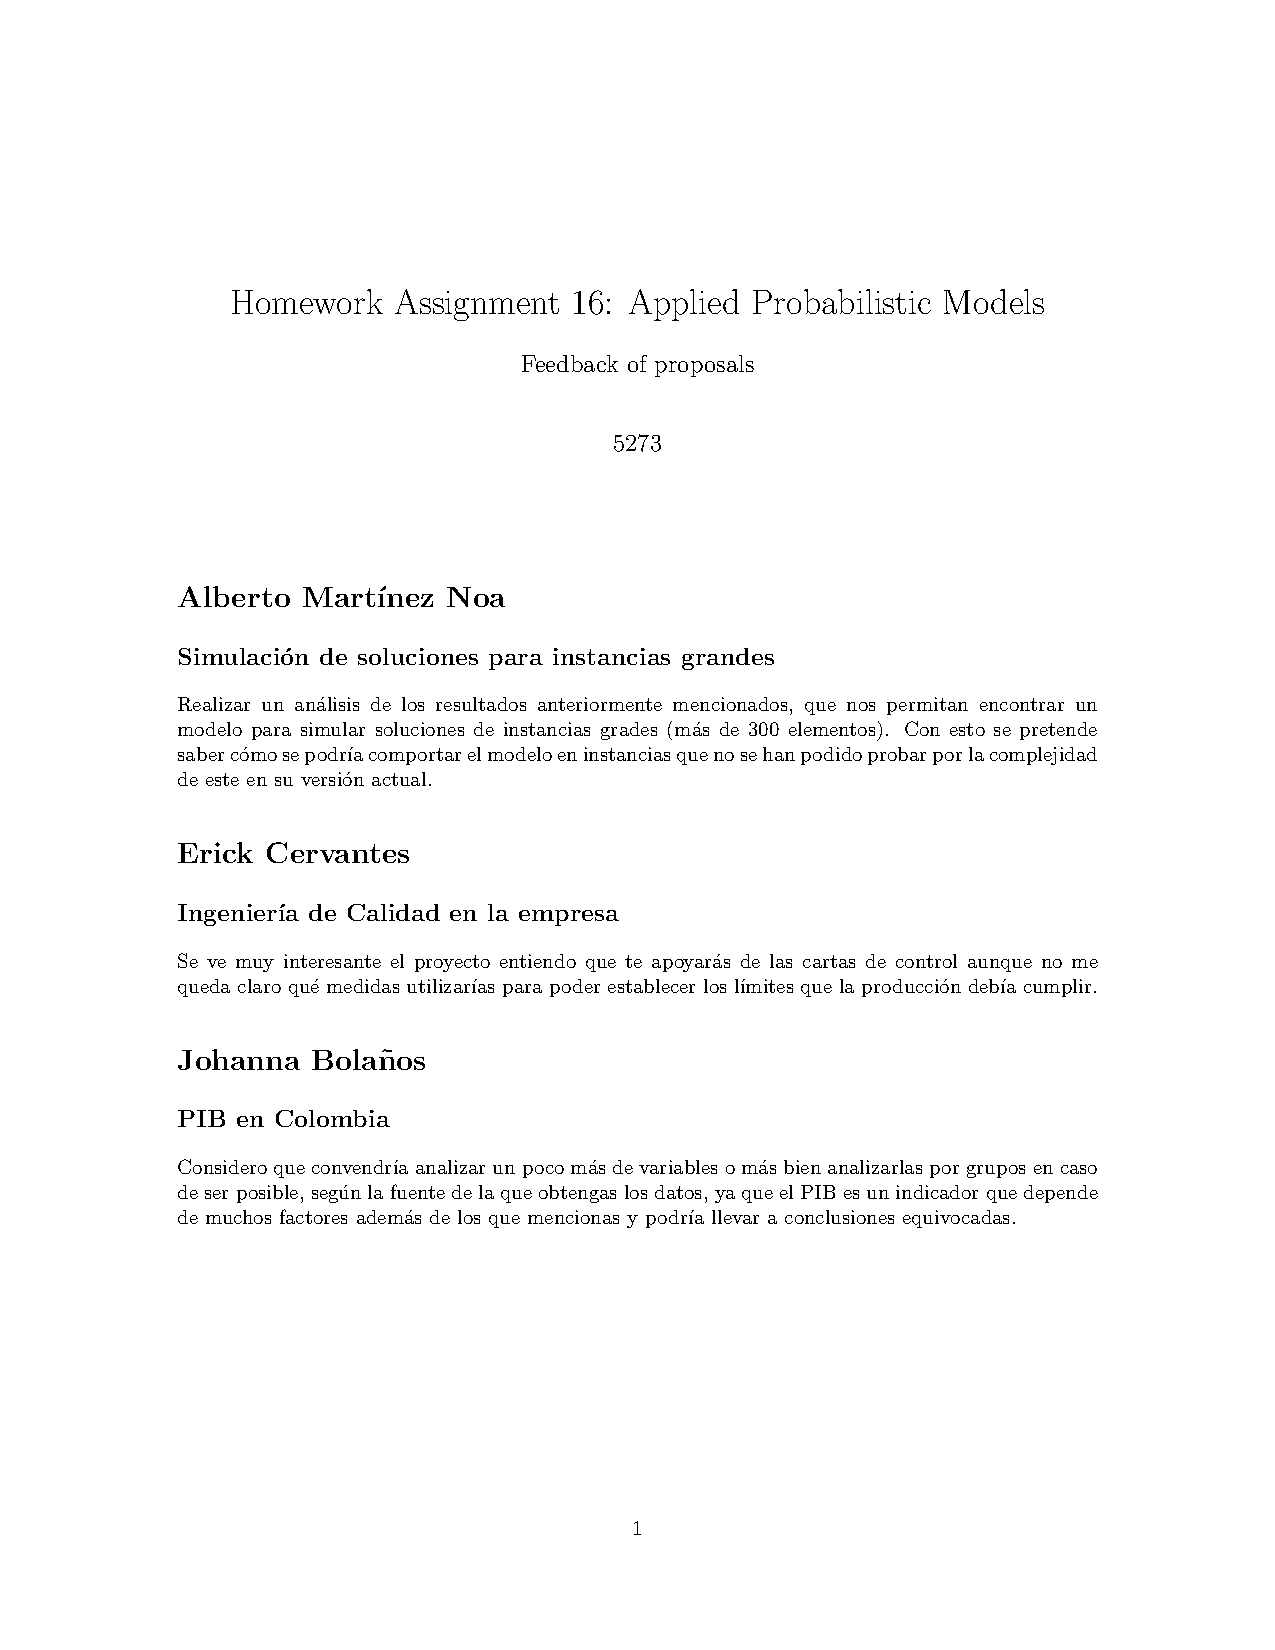
\includepdf[pages=-]{/Users/oscarhernandezlopez/Documents/GitHub/probability-in-R/assignment16/as16.pdf}
	
\end{document}